In this chapter, we briefly discuss the machine learning and computer vision concepts that have been used in the thesis.
\section{Machine Learning Concepts}
\label{sec_machine_learning_tools}

\subsection{Principal Component Analysis}
\label{subsec_pca}

Principal Component Analysis({\sc pca}) is a very popular dimensionality reduction approach proposed by Hotelling~\cite{hotelling}. Apart from dimensionality reduction, {\sc pca} is also used for data visualization, feature extraction and lossy data compression~\cite{prml}. 
{\sc pca} is the projection of data onto a orthogonal set of basis vectors such that the variance of the data after the projection is maximized. These basis vectors are obtained by solving an eigenvalue problem involving the covariance matrix of the data samples.

Consider a dataset consisting of $n$ observations ${x_1, x_2, ...x_n}$ such that $x_i \in R^d$. Let the first principal component be obtained by projecting the data along $u_1$, i.e. the direction of maximum variance of the data. The variance of the data along the direction $u_1$ can be represented as 

\begin{equation}\label{eq_pca1}
u_1^TSu_1
\end{equation} 
where $S$ is the covariance matrix of the observations given by

\begin{equation}\label{eq_pca2}
S= \frac{1}{n} \sum \limits_{i=1}^{n} x_i x_i^T.
\end{equation} 
Here the column vectors $x_i$ have been centered around the dataset mean. In order to maximize the variance given in Equation~\ref{eq_pca1}, we need to maximize the objective with respect to $u_1$. However, unconstrained maximization of this objective will result in $u_1$ having very large magnitude. In order to keep the $l_2$ norm of $u_1$ under check, a unit norm constraint is added to objective. This constrained objective can be converted to an unconstrained one using the method of Lagrange multipliers . Using this approach, the unconstrained objective can be rewritten as

\begin{equation}\label{eq_pca3}
u_1^TSu_1 \hspace{.2cm} + \lambda_1(1-u_1^Tu_1),
\end{equation}
where $\lambda_1$ is the Lagrange multiplier. This objective can be maximized by setting its derivative with respect to $u_1$ as zero. This results in the following eigenvalue problem

\begin{equation}\label{eq_pca4}
Su_1 = \lambda_1 u_1.
\end{equation}
Hence $u_1$ is the eigenvector of $S$ which corresponds to its largest eigenvalue. The other eigenvectors can be found similarly with added constraint that the eigenvectors must be orthogonal to one another. We have described the maximum variance formulation for {\sc pca} as in Bishop~\cite{prml}.

\subsection{Support Vector Machine}
\label{subsec_svm}

Consider a binary classification problem where any feature vector $x \in R^d$ and corresponding class labels can be $y \in \{1, -1 \}$. Support vector machine({\sc svm}) constructs a decision surface in the form of a separating hyperplane: 

\begin{equation}\label{eq_svm1}
w^Tx + b = 0
\end{equation}
so that the positive and the negative examples are separated by the hyperplane. There can be an infinite number of hyperplanes which separates the positive \& the negative examples(in case the data is linearly separable). Out of all such hyperplanes, {\sc svm} picks the hyperplane which maximizes the margin between the examples in the positive and the negative class.
Such a hyperplane must satisfy:
\begin{eqnarray}
w^Tx_i + b \geq 1 \hspace{.2cm} \mbox{for} \hspace{.2cm} y_i = 1, \\
w^Tx_i + b < -1 \hspace{.2cm} \mbox{for} \hspace{.2cm} y_i = -1 
\end{eqnarray}
The margin of separation $\rho$, between the positive and the negative examples is given by
\begin{equation}
\rho = \frac{2}{|w|}
\end{equation}
The margin maximizing hyperplane can be found by solving the following constrained optimization problem
\begin{equation}
\min_{w,b}\frac{1}{2}w^Tw \hspace{.3cm} \mbox{subject to} \hspace{.3cm} y_i(w^Tx_i + b) \geq 1.
\end{equation}
The above optimization problem is convex and hence, a unique hyperplane exists which is a global solution of the above constrained optimization problem. However, it turns out that many real world datasets are not linearly separable. Hence, in such a case, any feasible solution for the above objective does not exist. A \textit{soft margin} version of {\sc svm} exists which can deal with such a scenario.

\subsubsection{Kernelized Approaches}
\label{subsub_kernelized_approaches}
Sometimes the patterns inherent in the data are not apparent from the original feature representation. In such scenarios, it is a common practice to do a linear or a non-linear mapping/transformation of the data so that after the transformation, the patterns in the data become more obvious. Kernel based approaches are a non-linear feature mapping approach which map the data points in the original space to its mapping in a Reproducing Kernel Hilbert Space({\sc rkhs}).

Consider feature vector $x \in R^d$. A kernel function $k$ is defined as
\begin{equation}\label{eqn:kernel1}
\begin{aligned}
k:X \times X \mapsto \mathbb{R}, \\
<x_i, x_j> \mapsto k(x_i, x_j),
\end{aligned}
\end{equation}
where $x_i$ and $x_j$ objects from $X$.
The kernel function $k$ is said to be positive definite if it satisfies the following properties
\begin{itemize}
\item $k$ is symmetric, i.e. $k(x_i, x_j)=k(x_j, x_i)$
\item $ \sum \limits_{i,j =1}^{n}\alpha_i \alpha_j k(x_i, x_j)\geq 0$, where $\alpha_i, \alpha_j \in \mathbb{R}$ and $n \in \mathbb{N}$
\end{itemize}
 If the kernel function is positive definite, then there exists some mapping function $\phi$ such that
 \begin{equation}\label{eqn:kernel2}
 <\phi(x_i), \phi(x_j)> = k(x_i, x_j),
 \end{equation}
 here $\phi$ is a mapping function which maps data points from original space to a Reproducing Kernel Hilbert Space({\sc rkhs}).

\subsubsection{Multiclass SVM}
\label{subsubsection_mc_svm}
Multiclass {\sc SVM } assigns the label to an instance where number of labels are more than two. The dominant approach for doing so is to reduce the multiclass problem into multiple binary classification problems. Building binary classifiers which distinguish between $(i)$ one of the labels and the rest (one-versus-all) or $(ii)$ between every pair of classes (one-versus-one). Classification of new instances for the one-versus-all case is done by a winner-takes-all strategy, in which the classifier with the highest output function assigns the class (it is important that the output functions be calibrated to produce comparable scores). For the one-versus-one approach, classification is done by a max-wins voting strategy, in which every classifier assigns the instance to one of the two classes, then the vote for the assigned class is increased by one vote, and finally the class with the most votes determines the instance classification.

\subsection{Artificial Neural Networks(ANN)}
\label{subsec:ANN}
Artificial Neural Network sometimes also abbreviated as Neural Networks is a computational model inspired from biological neural networks. \textit{Dr. Robert Hecht-Nielsen} inventor of first neuro computer defines neural network as - \\
``...\textit{a computing system made up of a number of simple, highly interconnected processing elements, which process information by their dynamic state response to external inputs.}". 
\subsubsection{Structure of Artificial Neural Networks} An ANN model Figure~\ref{fig:ann_diag01} encompass three different layers input layer, hidden layer and output layer.\\

\begin{figure}[h]
\centering
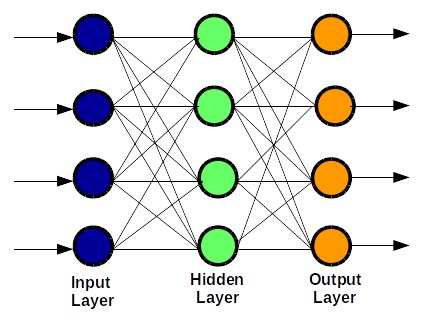
\includegraphics[width=12cm,height=9cm]{figures/ann_diag01.png}
\caption{Figure is decepting a general ANN model and different layers.}
\label{fig:ann_diag01}
\end{figure}

\textbf{Input Layer:} All the inputs are fed into the model through this layer. The Input layer is a communication medium with the external environment that feed a pattern to the ANN.

\textbf{Hidden Layer:} Hidden layer is a group of neurons combined with the activation function\cite{activation_function} is an intermediate layer between the input and output layer. The job of this layer is process the input from its previous layer and pass the extracted data to next layer. Many researches has been conducted for evaluating the number of neurons in the hidden layer but still none of them was successful in finding the accurate result. Also there can be multiple hidden layers in an ANN model. Number of hidden layer depend upon the complexity of the input data. If we have a data which can be separated linearly, then there is no need of hidden layer as the activation function can be implemented to input layer which can solve the problem. But in case of data is non-linear and problems deals with complex decisions, we can use multiple hidden layers based on the degree of complexity of the problem. Increasing the number of layers will not always result into high accuracy. A stage comes when the accuracy becomes constant or falls with an extra added layer.
Also, we should calculate the optimal number of neurons for each network. If the number of neurons are less as compared to the complexity of the problem data then there will be very few neurons in the hidden layers to adequately detect the signals in a complicated data set. Whereas a greater number of neurons present in ANN may lead to overfitting of the model. In-order to tune the number of hidden layers and neurons there are some empirically-derived rules-of-thumb, of these, the most commonly relied on is, \textit{``the optimal size of the hidden layer is usually between the size of the input and size of the output layers" - Jeff Heaton}\cite{heaton2008introduction}.

\textbf{Output Layer:} The output layer of the neural network is the set of results generated by the previous layer. The number of neurons in output layer should be directly related to the type of work that the neural network was performing. To determine the number of neurons in the output layer, first consider the intended use of the neural network. 

\textbf{Working of ANN:} In the Figure~\ref{fig:ann_diag01} each connection between two neurons indicates the flow of the information. Each connection has there correspondig weights which control the signal intensity between two neurons. If the network generates desired result then there is no need of weight adjustment else weight adjustment is carried out by using Back Propagation Algorithm.

\textbf{Back Propagation Algorithm:} It is the training algorithm used to efficiently train ANN. It learn by example and adjust weight of neurons so that it can produce desired output from the trained model.

\subsection{Nearest Neighbors}
\label{subsec:Nearest Neighbors}
Nearest neighbors are one of the most classifiers, possibly because it does not involve any training. This technique simply consists of storing all the labeled training examples and given a test images, the label of closest training sample(or majority label of k-neighbors) is assigned to the test image. Nearest neighbors can be kernelized or coupled with metric learning~\cite{lmnn}.


For classification techniques such as {\sc svm}, only a single weight vector needs to be stored per class(in a one-vs-rest setting), however, a nearest neighbor classification strategy typically consists of storing all the training samples. This is one of the major demerits of nearest neighbors. 


\subsection{Random Walks on Graphs}
Let $G$ be a graph or digraph with the additional assumption that if $G$ is a directed graph, then $deg^+(v) > 0$ for every vertex $v$. Now consider an object placed at vertex $v_j$ . At each stage the object must move to an adjacent vertex. The probability that it moves to the vertex $v_i$ is $ \frac{1}{deg(v_j)}$ or 
$ \frac{1}{deg^+(v_j)}$ if $(v_j , v_i)$ is an edge on $G$ and $G$ is a graph or directed graph, respectively. Otherwise the probability is $0$. Therefore if we define as

\[
  m_{ij}=\begin{cases}
               \frac{1}{deg(v_j)} \quad \text{left if $(v_j , v_i)$ is an edge in the graph $G$}  \\ 
               \frac{1}{deg^+(v_j)} \quad \text{left if $(v_j , v_i)$ is an edge in the directed graph $G$}  \\ 
               0 \quad \text{otherwise}
            \end{cases}
\]

Then $M = (m_{ij})$ is a Markov matrix. Note that the roles of $i$ and $j$ are reversed as we need the columns of $M$ to sum to 1. As each stage occurs, a sequence of adjacent vertices is produced. This sequence represents the position of the object at a given stage. Moreover this sequence is a walk in the graph. We call such a walk a random walk on the graph or digraph $G$. Using the Markov matrix, we see that the $i, j$ entry of $M^k$
represents the probability that a random walk of length $k$ starting at vertex $v_j$ , ends at the vertex $v_i$. The steady-state vector will correspond to the probability of being at a given vertex after a sufficient number of random walks. The above random walks on graph definition is cited from \cite{random_walks}.

\subsection{Evaluation Measures}
\textbf{$k$-fold cross-validation:} We used $k$-fold cross validation technique to do the analysis of our experiments. In $k$-fold cross-validation, the original sample is randomly partitioned into $k$ equal sized subsamples. Of the k subsamples, a single subsample is retained as the validation data for testing the model, and the remaining $k-1$ subsamples are used as training data. The cross-validation process is then repeated $k$ times(the folds), with each of the $k$ subsamples used exactly once as the validation data. The k results from the folds can then be averaged(or otherwise combined) to produce a single estimation. The advantage of this method over repeated random sub-sampling is that all observations are used for both training and validation, and each observation is used for validation exactly once.\\
The above definition of $k$-fold cross validation is taken from Wiki source \cite{cross_validation} .
\begin{figure}[h]
\centering
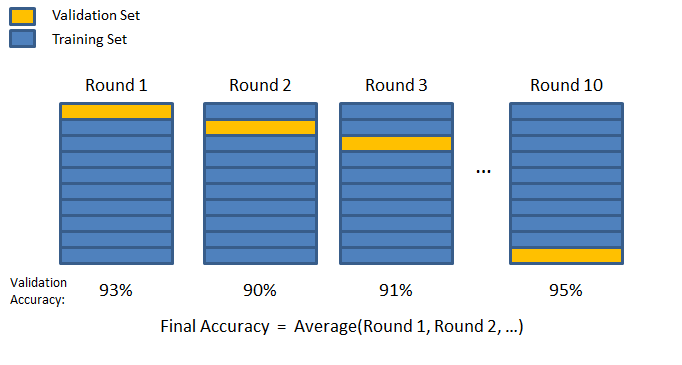
\includegraphics[width=\columnwidth,height=9cm]{figures/k_fold_cross_validation.png}
\caption{The training set is split into $k$ smaller sets and a model is trained using $k-1$ of the folds as training data. The resulting model is validated on the remaining part of the data. The performance measure reported by $k$-fold cross-validation is then the average of the values computed in the loop.}
\label{fig:k_fold_cross_validation}
\end{figure}

\section{Computer Vision Concepts}
\subsection{Bag Of Words}
The Bag-of-Words (BoW) methodology was first proposed in the text retrieval domain problem for text document analysis, and it was further adapted for computer vision applications \cite{bosch_best}. For image analysis, a visual analogue of a word is used in the BoW model, which is based on the vector quantization process by clustering low-level visual features of local regions or points, such as color, texture, and so forth. Below is the details description of the Bow methodology by Tsai \cite{tsai2012bag}.

To extract the BoW feature from images involves the following steps: $(i)$ automatically detect regions/points of interest, $(ii)$ compute local descriptors over those regions/points, $(iii)$ quantize the descriptors into words to form the visual vocabulary, and $(iv)$ find the occurrences in the image of each specific word in the vocabulary for constructing the BoW feature (or a histogram of word frequencies). Figure \ref{fig:bow_flow}(courtesy \cite{tsai2012bag}) describes these four steps to extract the BoW feature from images.

\begin{figure}[h]
\centering
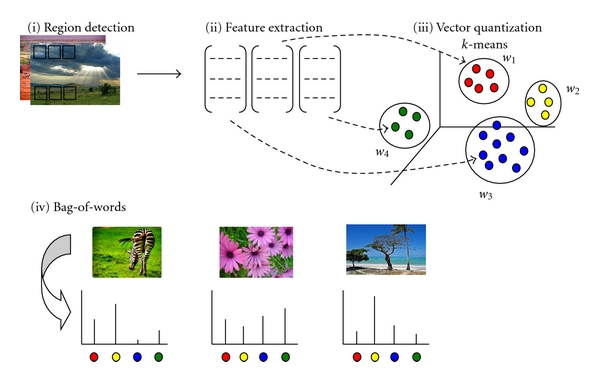
\includegraphics[width=\columnwidth,height=9cm]{figures/bow_flow.jpg}
\caption{Steps for constructing the bag-of-words for image representation. In first and second step finding the interest region and feature extractions are performed. While in third and fourth step clustering of features and histogram representation of the images are done.}
\label{fig:bow_flow}
\end{figure}

The BoW model can be defined as follows. Given a training dataset $D$ containing $n$ images represented by $D = d_1, d_2,..d_n$, where $d$ is the extracted visual features, a specific unsupervised learning algorithm, such as $k-means$, is used to group $D$ based on a fixed number of visual words $W$ (or categories) represented by $W= w_1, w_2,..w_v$, where $V$ is the cluster number. Then, we can summarize the data in a $V \times N$ co-occurrence table of counts $N_{ij}=n(w_i,d_j)$, where $n(w_i,d_j)$ denotes how often the word $w_i$ occurred in an image $d_j$.

\subsubsection{Interest Point Detection}
The first step of the BoW methodology is to detect local interest regions or points. For feature extraction of interest points (or keypoints), they are computed at predefined locations and scales. Several well-known region detectors that have been described in the literature are discussed below \cite{mikolajczyk2005local, tuytelaars2008local}.

\begin{enumerate}
\item Harris-Laplace regions are detected by the scale-adapted Harris function and selected in scale-space by the Laplacian-of-Gaussian operator. Harris-Laplace detects corner-like structures.

\item DoG regions are localized at local scale-space maxima of the difference-of-Gaussian. This detector is suitable for finding blob-like structures. In addition, the DoG point detector has previously been shown to perform well, and it is also faster and more compact (less feature points per image) than other detectors.

\item Hessian-Laplace regions are localized in space at the local maxima of the Hessian determinant and in scale at the local maxima of the Laplacian-of-Gaussian.

\item Salient regions are detected in scale-space at local maxima of the entropy. The entropy of pixel intensity histograms is measured for circular regions of various sizes at each image position.

\item Maximally stable extremal regions (MSERs) are components of connected pixels in a thresholded image. A watershed-like segmentation algorithm is applied to image intensities and segment boundaries which are stable over a wide range of thresholds that define the region.
\end{enumerate}

\subsubsection{Local Descriptors}
In most studies, some single local descriptors are extracted, in which the Scale Invariant Feature Transform(SIFT) descriptor is the most widely extracted \cite{lowe2004distinctive}. It combines a scale invariant region detector and a descriptor based on the gradient distribution in the detected regions. The descriptor is represented by a 3D histogram of gradient locations and orientations. The dimensionality of the SIFT descriptor is 128. SIFT was found to work best 
\cite{quelhas2007thousand, mikolajczyk2005local, mikolajczyk2005performance, zhang2007local}. SURF, ORB and BRISK few more widely used descriptors.

\subsubsection{Visual Word Generation/Vector Clustering}
When the keypoints are detected and their features are extracted, such as with the SIFT descriptor, the final step of extracting the BoW feature from images is based on vector quantization. In general, the $k-means$ or $hierarchical$ $k-means$ clustering algorithm is used for this task, and the number of visual words generated is based on the number of clusters(i.e.,). Jiang et al. \cite{jiang2010representations} conducted a comprehensive study on the representation choices of BoW, including vocabulary size, weighting scheme, such as binary, term frequency(TF) and term frequency-inverse document frequency (TF-IDF), stop word removal, feature selection, and so forth for video and image annotation.

\subsubsection{Building Inverted Index}
To perform large-scale image retrieval, Bag of Features methods require efficient indexing strategies and the ability to handle large vocabularies. An inverted index method for indexing the gallery term vectors is one where each term records the images in which it appears, along with the weight for each image. If each image yields approximately 2,000 interest points and the vocabulary size is $10K$ terms, then the resulting term vector (assuming no multiple/soft assignments) will have at most $20\%$ of its entries as non-zero. In a larger system with a vocabulary of $100K$ to $1M$ terms, the term vectors will be even sparser.

\subsubsection{Query Handling}
A simple approach to ranking query results is to compute the distance between the query
vector and the term vectors of each gallery image, requiring an $O(N)$ computation in term
of the number of gallery images. The majority of those images are likely to have very few
terms in common due to the sparsity of the vectors, however. Instead, one can look at each
non-zero term in the query vector and get the list of images in which that term appears via
the inverted index. The normalized $L_p$ distance to each image discovered in the inverted index can be computed incrementally as the inverted index is traversed, such as demonstrated in \cite{nister2006scalable}. While the worst case complexity remains $O(N)$, there is a huge speed improvement for the average case. Inverted indexes are used in all contemporary BoF-based image retrieval methods that were surveyed in the above report.


\subsection{Trifocal Tensor}
\textbf{Trifocal Geometry:} Finding the correspondence among the image primitives (points or lines) over multiple views
is recognized as a fundamental problem in computer vision. Assume we have three images
captured by three calibrated cameras with the known extrinsic calibration(camera positions in Euclidean space) 
and the intrinsic parameters (camera calibration information). Figure \ref{fig_trifocal_tensor} shows the geometry of three cameras. Their optical
centers are denoted by $C$, $C'$ and $C''$. A $3D$ point $X$ in Euclidean space has its
unique image on the image plane of each camera at where the ray linking the point
to the camera optical center intersects the plane. However the opposite is not true
since the image point can be the projection of any $3D$ point on that ray. The nonzero scale factor $\lambda$ in the equation \ref{eq_camera_world_point} explains this ambiguity. The Euclidean camera is defined by a $3\times4$ camera matrix $P=K[R|t]$.

\begin{figure}[t]
\centering
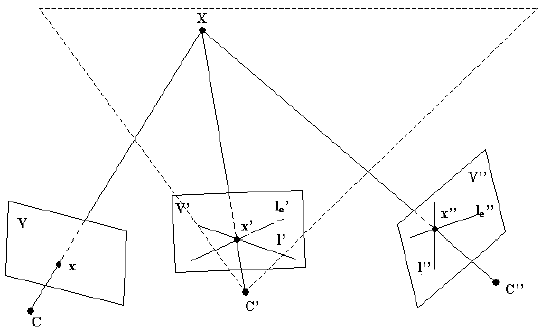
\includegraphics[width=12.5cm,height=8cm]{figures/trifocal_tensor_01.png}
\caption{Trifocal geometry of three views. $X$ is a $3D$ point viewed from three camera having optical center $C$, $C'$ and $C''$.}
\label{fig_trifocal_tensor}
\end{figure}

\begin{equation}
	P^P_i = H^P_j
\label{eq_projective_transformation}
\end{equation}


The $3 \times 3$ camera calibration matrix $K$ contains the intrinsic parameters of the specific camera. The camera's pose with
respect to the world coordinate system is represented by $3 \times 3$ rotation $R$ and $3D$ vector translation $t$. The projection from $3D$ point $(X;Y;Z)$ to image point $(x;y)$ is up to a scale. The scale ambiguity can be overcome by having correspondences for a feature in two views. The $3D$ point $X$ can then be reconstructed by means of triangulation using the point correspondence pair $x$ and $x'$ on view $V$ and $V'$. Then this point can
be re-projected into the third view $V''$ to find out where the image coordinate of this $3D$ point should appear on that view. This process $x$, $x \rightarrow x''$ is called transfer, and it can be done with at least one calibrated camera and correspondences across two views. For un-calibrated cameras no transformation between an image point and a ray in Euclidean space is provided because their intrinsic and extrinsic parameters are unknown.
\begin{equation}
 \lambda  \begin{pmatrix}
    	x \\
    	y \\
    	1 \\
    \end{pmatrix}
    = 
    P \begin{pmatrix}
   		X \\
   		Y \\
   		Z \\
   		1 \\
    \end{pmatrix}
\label{eq_camera_world_point}
\end{equation}

In this case the cameras are defined to be projective cameras$(K=I)$ and any one can be replaced by another. The $3D$-to-$2D$ projection $P^p$ becomes camera independent. The projective spaces where such projections take place are all equivalent since they can align to each other only by a $3D$ projective transformation
($4 \times4$ matrix $H$)\cite{hartley2003multiple}.

\begin{equation}
	P^P_i = H^P_j
\label{eq_projective_transformation}
\end{equation}

It is the relative camera position that determines the transformation between two projective spaces. Usually when more than one camera are considered, a normalized camera coordinate system is used and one of 
cameras is $P = [I|0]$. Consequently the positions of other cameras in this system, and the extrinsic camera parameters are all that is necessary to define the camera projection matrices. Therefore even when
the three cameras mentioned above are not calibrated, image correspondences can still be transferred from two views to the third. As will be discussed in the next section, it is possible to define the projective geometry of the three cameras by a trifocal tensor. When the tensor is computed the transfer can be done directly by it
without computing an intermediate $3D$ point. Since this removes the need of camera calibration, the trifocal tensor has been recognized an important tool for processing three views.

It needs to be pointed out that corresponding image points on three views are also related by epipolar geometry. The ray projected from one image point will be viewed as a line in another view(called the epipolar line). The relation between image correspondences of a view pair is described by a $3 \times 3$ fundamental matrix, \textit{i.e} $x'^{T}F_{12}x=0$ of view $i$ and $j$. The three views can be registered together in a
pair-wise manner. Again given a pair of image correspondence$(x, x')$, intersecting their epipolar lines on the third view should show the image position of the $3D$ point. However, if the point $X$ is in the trifocal plane defined by the optical centers $C$, $C'$ and $C''$. or if the centers are aligned, it is impossible to determine if three image points belong to a single $3D$ point by epipolar geometry. Such ambiguity can be avoided
by using a trifocal tensor since it provides a more accurate and stable description of three views' geometry than the fundamental matrices between each pair of views.\\

\textbf{Trifocal Tensor:} The trifocal tensor is expressed by a set of three $ 3 \times 3$ matrices,$[T_i]$, $i=1,2,3$. It describes the projective geometric relations of image triplets taken from three cameras. Considering a view triplet, if the camera matrix of the first view is in canonical form, $P_1 = [I|0]$, and the camera matrices of the other two views are expressed as $P_2 = [A|e']$, $P_3 = [B|e'']$, where $A$ and $B$ are $3 \times 3$ matrices, and $e'$ and $e''$ are the epipoles corresponding to the image of the center of the first camera on the image plane of the second and third cameras respectively, then the $3\times3\times3$ trifocal tensor
can be denoted as $T  = [T_1,T_2,T_3] ^ T$, with:

\begin{equation}
	T_i = a_ie''^T - e'b_i^T 
\label{eq_trifocal_relation}
\end{equation}

The equation \ref{eq_trifocal_relation} presents a straightforward way to construct the trifocal tensor from the camera matrices.
\newpage

%\section{Dataset and Evaluation measures}
%
%\subsection{Dataset}
%\textbf{Video Runs:} Video run dataset consist of 10 video runs of a 600m long path. We used contour action camera at resolution $1920 \times 1080$ at $30 fps$ to capture the videos. The device also had inbuilt \gps sensor which recorded the \gps signal at $1Hz$ and loosely synchronized with video frames. Data was collected over 10 different days in evening at peak traffic hours to ensure urban environment setting.\\
%
%\textbf{Mobile Sensor Dataset:} We created and Android application in order to built mobile sensor dataset. Application used to log the the accelerometer sensor data, screen on duration, internet,
%CPU and RAM usage of the device at every half an hour interval over the period of 6 working days.
%The class label of an interval is decided based on the internet usage by the user within the time window. We ran the application for a total of over 6 working days on smart phones, which
%resulted in 310 labeled feature samples.
%
%
%%\textbf{Heritage Site Story Telling:} To show case our story telling work we choosen Qutub Shahi Tomb, Ibrahim Bag, Hyderbad. Qutub Shahi Tomb is a popular world heritage site spread in  $170000$ square meter area. We captured $1077$ images for $15$ distinct sites ranging from $30$ to $80$ images for each site depending on the area it covers. We recorded \gps signals at $1Hz$ and capture videos
%%with resolution $1920 \times 1080$ at $30 fps$. We also collected stories for distinct scene 
%%and details from the monuments, adding more to narratives we even collected the famous stories related to the sites from the web.
%
%\subsection{Evaluation Measures}
%\textbf{$k$-fold cross-validation:} We used $k$-fold cross validation technique to do the analysis of our experiments. In $k$-fold cross-validation, the original sample is randomly partitioned into $k$ equal sized subsamples. Of the k subsamples, a single subsample is retained as the validation data for testing the model, and the remaining $k$ − 1 subsamples are used as training data. The cross-validation process is then repeated $k$ times(the folds), with each of the $k$ subsamples used exactly once as the validation data. The k results from the folds can then be averaged(or otherwise combined) to produce a single estimation. The advantage of this method over repeated random sub-sampling is that all observations are used for both training and validation, and each observation is used for validation exactly once.\\
%The above definition of $k$-fold cross validation is taken from Wiki source \cite{cross_validation} .
%
%\newpage



